\documentclass[12pt]{article}
\usepackage[margin=1in]{geometry}
\usepackage{setspace}
\usepackage{booktabs}
\usepackage{threeparttable}
\usepackage{pgfplots}
\usepackage{caption}
\usepackage[round,authoryear]{natbib}
\pgfplotsset{compat=1.17}
\onehalfspacing

\title{Kept Aloft: A State Rescue and the Route Network of a Regional Airline\\[6pt]
\normalsize\textbf{SYNTHETIC TEST PAPER, NOT REAL RESEARCH}}
\author{Ilse Varnholt\\Department of Strategy, University of Port Aubrin}
\date{Working paper, September 2026}

\begin{document}
\maketitle

\begin{abstract}
\noindent
When a government rescues a failing firm, it changes what the firm can afford to do next. We study a state rescue of Tarnwick Regional Airways, a mid-sized carrier in the Republic of Estmere, in 2014. Using a synthetic control built from the 15 other scheduled domestic carriers and six annual pre-rescue years, we estimate that the rescue raised Tarnwick's route count by 13.2 routes a year on average over 2014 to 2019, about a fifth of its pre-rescue network. The permutation p-value is 0.02. Augmented synthetic control and synthetic difference-in-differences estimates are close to the main estimate. The results suggest that a rescued firm uses its protected position to expand rather than to retrench, and that rescues reshape the competitive position of the rescued firm's rivals.
\end{abstract}

\noindent\textbf{Keywords:} state aid; soft budget constraint; airlines; synthetic control; firm scope

\newpage

\section{Introduction}

Governments rescue firms more often than the strategy literature acknowledges. A rescue can take the form of an equity injection, a loan guarantee, or a debt write-down, and it usually comes with conditions on employment or service. The strategic question is what the rescued firm does with the room the rescue gives it. One view holds that a rescued firm retrenches: it closes unprofitable operations, repays its creditors, and returns to a narrower core. A second view holds that a rescue relaxes the budget constraint on managers, who then pursue growth that the market would not have financed.

Airlines are a useful place to study this question. Route networks are visible, they change every season, and the decision to open or close a city pair is a strategic choice about scope. Regional carriers are also frequent recipients of state support, because they serve peripheral communities that governments want connected.

We study one rescue. In February 2014 the government of the Republic of Estmere took a 49 percent equity stake in Tarnwick Regional Airways and guaranteed a loan that covered the carrier's aircraft lease obligations for five years. Tarnwick had lost money in four of the previous five years. The rescue came with a condition that Tarnwick keep serving eleven named peripheral airports, but it placed no limit on new routes.

Because only one carrier was rescued, a comparison with a regression on many treated firms is not available. We use the synthetic control method \citep{abadie2003, abadie2010, abadie2021}, which builds a counterfactual Tarnwick as a weighted average of carriers that were not rescued. \citet{fremeth2016} show how the method suits organizational research with one or a few treated firms. The donor pool is the 15 other scheduled domestic carriers that operated in Estmere throughout 2008 to 2019. The outcome is the number of scheduled city-pair routes a carrier operates in a year.

We find that Tarnwick's route network grew well beyond its synthetic counterpart after the rescue. By 2019 Tarnwick operated 86 routes, while the synthetic Tarnwick operated 68. The average post-rescue gap is 13.2 routes. The effect is not driven by any single donor, it does not appear when we move the rescue date back three years, and augmented synthetic control, synthetic difference-in-differences, and a simple difference-in-differences comparison all give estimates of the same sign and similar size.

The paper makes two contributions. First, it gives firm-level evidence that a rescue leads to expansion of scope rather than retrenchment, at least for this carrier. Second, it shows how a single rescue can alter the route decisions of the rescued firm's rivals, which has implications for competition policy on state aid.

\section{Setting and hypothesis}

\subsection{Domestic aviation in Estmere}

Estmere is a country of about eleven million people with a mountainous interior and a long coastline. Domestic air travel links the capital, Port Aubrin, with provincial cities and with small airports in the interior. In 2008 eighteen carriers held scheduled domestic operating licenses. The Estmere Civil Aviation Authority (ECAA) publishes each carrier's filed schedule twice a year, listing every city pair the carrier serves.

The carriers differ in size and geography. The largest operated 118 routes on average over 2008 to 2013, and the smallest operated 22. Most carriers concentrate their departures at one hub. Tarnwick's hub is Selmar in the southwest, and it competes on some city pairs with four other carriers: Pelagia Airways, Sundra Express, Norvik Air, and Tessaly Air.

\subsection{The Tarnwick rescue}

Tarnwick entered financial distress after 2009, when fuel prices rose and a domestic recession cut demand. Its lessors threatened to recall aircraft in late 2013. Negotiations with the Ministry of Transport became public in November 2013, and the rescue was announced on 11 February 2014. Tarnwick filed both of its 2013 seasonal schedules with the ECAA by August 2013, before the negotiations became public, so its 2013 route count predates any public news of the rescue. The package had three parts: an equity injection for a 49 percent state stake, a five-year state guarantee on lease payments, and a service obligation for eleven peripheral airports. No other Estmere carrier received state aid between 2008 and 2019.

\subsection{Hypothesis}

A rescue removes the threat of liquidation for a period and signals that the state will support the firm again if needed. Managers of a rescued firm face a softer budget constraint. They can open routes whose expected returns would not satisfy a private lender, because the downside falls partly on the state. Routes are also a visible way to show the state that the rescue preserved connectivity, which raises the political value of the firm. Both arguments point to expansion.

\begin{quote}
\textit{Hypothesis 1.} A state rescue increases the number of routes the rescued carrier operates, relative to what it would have operated without the rescue.
\end{quote}

\section{Data}

We assembled a carrier-year panel from the ECAA schedule filings for 2008 to 2019. A route is a city pair, counted once regardless of direction, that the carrier served in at least one of the two schedule seasons of the year. We stop in 2019 because the 2020 pandemic suspended most domestic service.

Two carriers that merged in 2012 are dropped from the donor pool, because the merger changed both networks at once. This leaves 16 carriers: Tarnwick and 15 donors. All 15 donors operated throughout 2008 to 2019, none received state aid, and none changed ownership in the period.

We measure three carrier characteristics from the ECAA fleet register and schedule filings. Fleet size is the number of aircraft on the carrier's operating certificate at year end. Fleet age is the mean age of those aircraft in years. Hub share is the percentage of the carrier's scheduled departures that leave from its busiest airport. Table~\ref{tab:desc} reports the pre-rescue means for Tarnwick and the donor pool. It also reports the standard deviation of the year-to-year change in route count, a measure of how volatile each carrier's network is.

\begin{table}[ht]
\centering
\begin{threeparttable}
\caption{Descriptive statistics, 2008 to 2013}
\label{tab:desc}
\begin{tabular}{lcccc}
\toprule
 & Tarnwick & \multicolumn{3}{c}{Donor pool (15 carriers)} \\
\cmidrule(lr){3-5}
 & & Mean & Min & Max \\
\midrule
Route count & 62.3 & 54.1 & 22.4 & 117.8 \\
Fleet size (aircraft) & 34.2 & 29.8 & 11.0 & 71.5 \\
Fleet age (years) & 11.8 & 10.4 & 6.1 & 16.9 \\
Hub share (percent) & 41.3 & 38.6 & 18.2 & 67.4 \\
SD of annual change in route count & 5.5 & 4.8 & 1.9 & 9.6 \\
\bottomrule
\end{tabular}
\begin{tablenotes}\footnotesize
\item Notes: Means over the six pre-rescue years 2008 to 2013. Donor columns report the mean, minimum, and maximum across the 15 donor carriers of each carrier's six-year mean. The last row is the standard deviation across years of the annual change in route count, computed for each carrier over 2009 to 2013. Source: ECAA schedule filings and fleet register.
\end{tablenotes}
\end{threeparttable}
\end{table}

Tarnwick's route count rose from 56 in 2008 to 68 in 2013, with a dip in 2011 during the recession. On each characteristic in Table~\ref{tab:desc}, Tarnwick lies inside the range of the donor pool and close to its mean.

\section{Method}

\subsection{Synthetic control}

Let carrier 1 be Tarnwick and carriers 2 to 16 the donors. The synthetic control estimator chooses nonnegative weights $w_2, \dots, w_{16}$ that sum to one so that the weighted average of the donors matches Tarnwick on a set of pre-rescue predictors \citep{abadie2010}. The estimated effect in year $t$ is Tarnwick's route count minus the weighted average of the donors' route counts. We have $T_0 = 6$ pre-rescue years (2008 to 2013) and six post-rescue years (2014 to 2019). The main estimate is the average of the six post-rescue gaps.

The predictors are fleet size, fleet age, and hub share, each averaged over 2008 to 2013, together with Tarnwick's route count in each of the six pre-rescue years, 2008, 2009, 2010, 2011, 2012, and 2013, entered as six separate predictors. Balance on fleet size, fleet age, and hub share matters in this setting because these characteristics drive a carrier's capacity to open routes; including them ensures that the synthetic Tarnwick resembles the actual carrier on its fundamentals and not only on its past route counts. The predictor weights are chosen by the standard data-driven procedure that minimizes the pre-rescue mean squared prediction error of the outcome. We fixed the predictor set and the donor pool before examining any post-2014 schedule data.

\subsection{Inference}

We use the in-space placebo procedure of \citet{abadie2010}. We reassign the rescue to each of the 15 donors in turn, fit a synthetic control for each placebo carrier from the remaining 15 carriers, and compute the ratio of post-rescue to pre-rescue root mean squared prediction error for every carrier. The ratio accounts for the fact that a placebo carrier with a poor pre-rescue fit will show large post-rescue gaps for mechanical reasons. We keep all 15 placebo runs; none is discarded for poor fit. The p-value is the share of the 16 carriers whose ratio is at least as large as Tarnwick's. This procedure is design-based. It asks how unusual Tarnwick's ratio is among the carriers in the sample and does not rest on a sampling distribution; since the rescue was not assigned at random, we read it as a measure of how extreme Tarnwick's post-rescue path is relative to the other carriers.

\subsection{Alternative estimators}

We report three alternative estimators beside the synthetic control. The augmented synthetic control method of \citet{benmichael2021} adds a ridge regression outcome model that corrects for any remaining imbalance in the pre-rescue fit. Its weights sum to one but can be negative, so it is not a plain synthetic control, and we label it separately. Synthetic difference-in-differences \citep{arkhangelsky2021} combines unit weights with time weights and allows a level difference between Tarnwick and its weighted donors. Finally, a simple difference-in-differences compares Tarnwick's change in mean route count from 2008--2013 to 2014--2019 with the same change for the unweighted donor average.

\section{Results}

\subsection{Main estimate}

Figure~\ref{fig:path} shows Tarnwick's route count and that of its synthetic control. The synthetic Tarnwick is a weighted average of four donors (Table~\ref{tab:weights}). The fit before 2014 is excellent: the synthetic carrier reproduces Tarnwick's route network year by year through the recession and recovery. After the rescue the two paths separate at once. Tarnwick opened routes every year from 2014 to 2019, reaching 86 routes in 2019. The synthetic Tarnwick grew slowly, from 64 routes in 2013 to 68 in 2019.

\begin{figure}[ht]
\centering
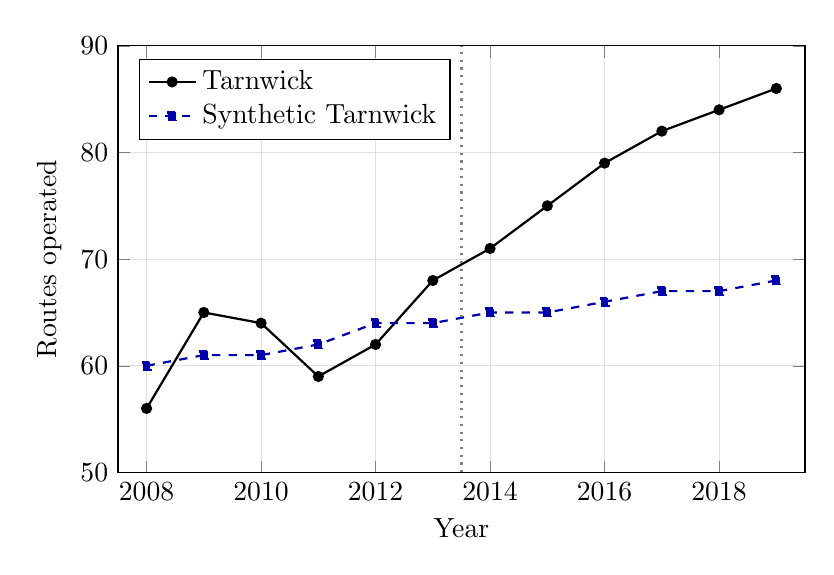
\begin{tikzpicture}
\begin{axis}[
  width=0.85\textwidth, height=7cm,
  xlabel={Year}, ylabel={Routes operated},
  xmin=2007.5, xmax=2019.5, ymin=50, ymax=90,
  xtick={2008,2010,2012,2014,2016,2018},
  x tick label style={/pgf/number format/1000 sep={}},
  legend pos=north west, legend cell align=left,
  grid=major, grid style={gray!25}
]
\addplot[thick, black, mark=*, mark size=1.6pt] coordinates {
(2008,56) (2009,65) (2010,64) (2011,59) (2012,62) (2013,68)
(2014,71) (2015,75) (2016,79) (2017,82) (2018,84) (2019,86)};
\addlegendentry{Tarnwick}
\addplot[thick, dashed, blue!70!black, mark=square*, mark size=1.4pt] coordinates {
(2008,60) (2009,61) (2010,61) (2011,62) (2012,64) (2013,64)
(2014,65) (2015,65) (2016,66) (2017,67) (2018,67) (2019,68)};
\addlegendentry{Synthetic Tarnwick}
\draw[gray, thick, dotted] (axis cs:2013.5,50) -- (axis cs:2013.5,90);
\end{axis}
\end{tikzpicture}
\caption{Route count, Tarnwick and synthetic Tarnwick, 2008 to 2019. The dotted line marks the rescue (February 2014).}
\label{fig:path}
\end{figure}

Figure~\ref{fig:gap} plots the gap between the two paths. The post-rescue gap grows from 6 routes in 2014 to 18 in 2019, and its average over the six post-rescue years is 13.2 routes. Tarnwick operated 62.3 routes on average before the rescue, so the effect is about a fifth of its pre-rescue network.

\begin{figure}[ht]
\centering
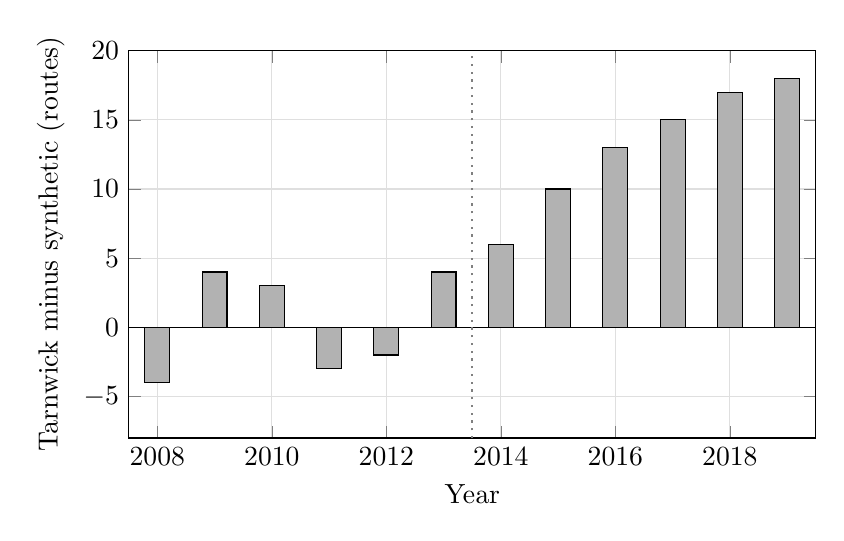
\begin{tikzpicture}
\begin{axis}[
  width=0.85\textwidth, height=6.5cm,
  xlabel={Year}, ylabel={Tarnwick minus synthetic (routes)},
  xmin=2007.5, xmax=2019.5, ymin=-8, ymax=20,
  xtick={2008,2010,2012,2014,2016,2018},
  ytick={-5,0,5,10,15,20},
  x tick label style={/pgf/number format/1000 sep={}},
  grid=major, grid style={gray!25}
]
\addplot[ybar, bar width=9pt, fill=gray!60, draw=black] coordinates {
(2008,-4) (2009,4) (2010,3) (2011,-3) (2012,-2) (2013,4)
(2014,6) (2015,10) (2016,13) (2017,15) (2018,17) (2019,18)};
\draw[black] (axis cs:2007.5,0) -- (axis cs:2019.5,0);
\draw[gray, thick, dotted] (axis cs:2013.5,-8) -- (axis cs:2013.5,20);
\end{axis}
\end{tikzpicture}
\caption{Gap between Tarnwick and synthetic Tarnwick, 2008 to 2019. Bars show Tarnwick's route count minus the synthetic control's route count in each year.}
\label{fig:gap}
\end{figure}

\subsection{Permutation inference}

Figure~\ref{fig:ratio} reports the ratio of post-rescue to pre-rescue root mean squared prediction error for Tarnwick and for each of the 15 placebo carriers. Tarnwick's ratio is 4.04, the largest of the 16 carriers. The next largest, for Halden Air, is 2.87. The permutation p-value is 0.02, significant at the 5 percent level. We therefore reject the null hypothesis that the rescue had no effect on Tarnwick's route count, in support of Hypothesis~1.

\begin{figure}[ht]
\centering
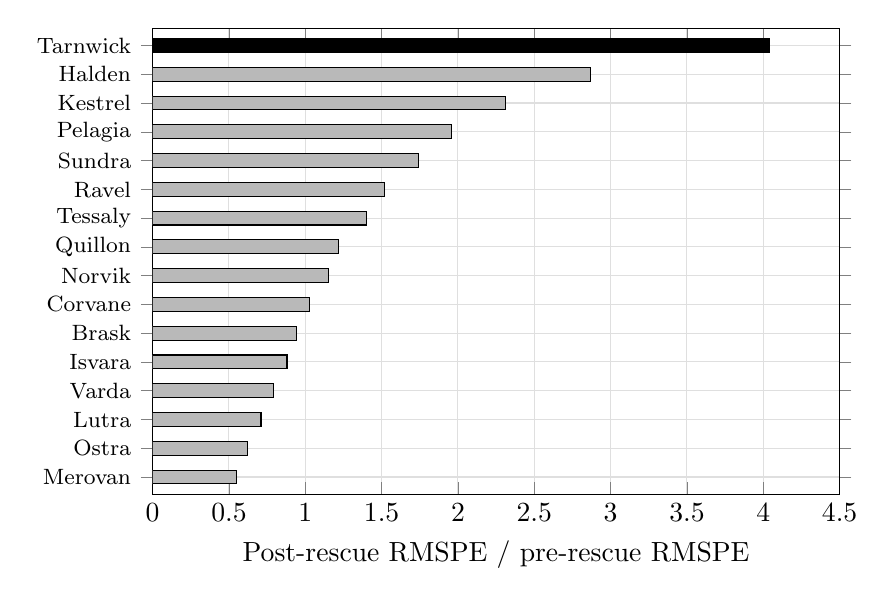
\begin{tikzpicture}
\begin{axis}[
  width=0.85\textwidth, height=7.5cm,
  xbar, bar width=5pt,
  xlabel={Post-rescue RMSPE / pre-rescue RMSPE},
  xmin=0, xmax=4.5,
  ytick={1,...,16}, bar shift=0pt,
  yticklabels={Merovan, Ostra, Lutra, Varda, Isvara, Brask, Corvane, Norvik, Quillon, Tessaly, Ravel, Sundra, Pelagia, Kestrel, Halden, Tarnwick},
  y tick label style={font=\footnotesize},
  enlarge y limits=0.04,
  grid=major, grid style={gray!25}
]
\addplot[fill=gray!55, draw=black] coordinates {
(0.55,1) (0.62,2) (0.71,3) (0.79,4) (0.88,5) (0.94,6) (1.03,7) (1.15,8)
(1.22,9) (1.40,10) (1.52,11) (1.74,12) (1.96,13) (2.31,14) (2.87,15)};
\addplot[fill=black, draw=black] coordinates {(4.04,16)};
\end{axis}
\end{tikzpicture}
\caption{Ratio of post-rescue (2014 to 2019) to pre-rescue (2008 to 2013) root mean squared prediction error, Tarnwick (black) and the 15 placebo carriers (gray). Each placebo carrier's synthetic control is fitted from the other 15 carriers with the same predictors as the main specification. No placebo run is discarded.}
\label{fig:ratio}
\end{figure}

\subsection{Donor weights and leave-one-out results}

Table~\ref{tab:weights} lists the donors that receive positive weight. Kestrel Regional carries 0.62 of the weight, Pelagia Airways 0.21, Sundra Express 0.11, and Brask Air 0.06. The weights sum to one. The other 11 donors receive zero weight. The last column marks the carriers that served at least one city pair in common with Tarnwick in 2013.

\begin{table}[ht]
\centering
\begin{threeparttable}
\caption{Synthetic control donor weights}
\label{tab:weights}
\begin{tabular}{lccc}
\toprule
Donor & Weight & Hub & Shares a city pair with Tarnwick \\
\midrule
Kestrel Regional & 0.62 & Varn (north) & No \\
Pelagia Airways & 0.21 & Selmar (southwest) & Yes \\
Sundra Express & 0.11 & Port Aubrin & Yes \\
Brask Air & 0.06 & Hollin (east) & No \\
\midrule
Total & 1.00 & & \\
\bottomrule
\end{tabular}
\begin{tablenotes}\footnotesize
\item Notes: Weights from the main synthetic control specification. The remaining 11 donors, including Norvik Air and Tessaly Air (both of which also share city pairs with Tarnwick), receive zero weight.
\end{tablenotes}
\end{threeparttable}
\end{table}

A weight of 0.62 on one donor means the counterfactual rests mainly on Kestrel. That has an advantage and a cost. The advantage is that the counterfactual is easy to read: synthetic Tarnwick is mostly Kestrel, a carrier of similar size (31.5 aircraft on average before 2014, against Tarnwick's 34.2), similar fleet age (12.4 years against 11.8), and similar hub share (44.0 percent against 41.3), operating in the north with no route overlap with Tarnwick. The cost is that the estimate depends on Kestrel having no shock of its own after 2014. We checked the ECAA records and found no ownership change, bankruptcy filing, fleet grounding, or state support for Kestrel in 2014 to 2019. Because Tarnwick lies inside the donors' range on every predictor in Table~\ref{tab:desc}, the synthetic control interpolates between observed carriers rather than extrapolating beyond them.

Table~\ref{tab:loo} reports the average post-rescue gap when we drop each positively weighted donor from the pool in turn and refit the weights. Dropping a zero-weight donor leaves the weights and the estimate unchanged, so we do not report those runs. Dropping Kestrel lowers the estimate to 11.9 routes; the new weights spread across Brask, Pelagia, and Corvane Airlines, and the pre-rescue path of the refitted synthetic Tarnwick is visually similar to Figure~\ref{fig:path}. Across the four runs the estimate stays between 11.9 and 13.4 routes.

\begin{table}[ht]
\centering
\begin{threeparttable}
\caption{Leave-one-out estimates}
\label{tab:loo}
\begin{tabular}{lc}
\toprule
Donor dropped & Average post-rescue gap (routes) \\
\midrule
None (main estimate) & 13.2 \\
Kestrel Regional & 11.9 \\
Pelagia Airways & 12.3 \\
Sundra Express & 12.7 \\
Brask Air & 13.4 \\
\bottomrule
\end{tabular}
\begin{tablenotes}\footnotesize
\item Notes: Each row drops one donor with positive weight in Table~\ref{tab:weights} and refits the synthetic control on the remaining 14 donors with the main predictor set. The estimate is the mean of the 2014 to 2019 gaps.
\end{tablenotes}
\end{threeparttable}
\end{table}

\subsection{In-time placebo}

If the synthetic control picks up a trend that has nothing to do with the rescue, it should also find an effect at a false date. We move the rescue back three years, to 2011, well before negotiations with the ministry became public in November 2013. We refit the weights using only the 2008 to 2010 data (route count in each of those three years plus the three characteristics averaged over 2008 to 2010) and compare Tarnwick with the refitted synthetic control over 2011 to 2013, the years before the true rescue. The placebo gaps are 1.8 routes in 2011, $-2.6$ in 2012, and 2.9 in 2013, an average of 0.7 routes. These gaps are within the size of the pre-rescue gaps in Figure~\ref{fig:gap} and far below the 13.2-route effect after the true date. The backdated synthetic control places 0.58 of its weight on Kestrel. Because the placebo window ends before the rescue was publicly discussed, it is not contaminated by anticipation.

\subsection{Alternative estimators}

Table~\ref{tab:alt} compares the main estimate with the three alternatives. The augmented synthetic control estimate is 12.1 routes. Its ridge correction assigns negative weights to two donors, Ravel Air ($-0.05$) and Quillon Air ($-0.03$); the positive weights sum to 1.08, so all weights sum to one. Because of the negative weights, the augmented estimator extrapolates slightly beyond the donors, and we report it as augmented synthetic control, not as synthetic control. The synthetic difference-in-differences estimate is 11.4 routes. The simple difference-in-differences estimate is 15.8 routes: Tarnwick's mean route count rose by 17.2 from 2008--2013 to 2014--2019, while the unweighted donor average rose by 1.4.

\begin{table}[ht]
\centering
\begin{threeparttable}
\caption{Synthetic control and alternative estimators}
\label{tab:alt}
\begin{tabular}{lcc}
\toprule
Estimator & Mean effect (routes) & Uncertainty \\
\midrule
Synthetic control (main) & 13.2 & See Section 5.2 \\
Augmented synthetic control (ridge) & 12.1 & \\
Synthetic difference-in-differences & 11.4 & (3.9) \\
Difference-in-differences & 15.8 & \\
\bottomrule
\end{tabular}
\begin{tablenotes}\footnotesize
\item Notes: One treated carrier (Tarnwick) and 15 donor carriers, 2008 to 2019. Augmented synthetic control follows \citet{benmichael2021}; two donors receive negative weights. Synthetic difference-in-differences follows \citet{arkhangelsky2021}; the standard error in parentheses is the jackknife standard error. Difference-in-differences compares Tarnwick with the unweighted donor average. We do not report a standard error for the augmented or difference-in-differences estimates.
\end{tablenotes}
\end{threeparttable}
\end{table}

For the synthetic difference-in-differences estimate we report the weights and regularization. The unit weights are more dispersed than the synthetic control weights: 11 of the 15 donors receive positive weight, and the largest, Kestrel, receives 0.19. The regularization parameter, set by the rule in \citet{arkhangelsky2021}, is 3.2. The time weights place 0.64 on 2013 and 0.36 on 2012 and zero on earlier years. The jackknife standard error is 3.9, which gives a t-statistic of 2.9, significant at the 1 percent level. The synthetic difference-in-differences result thus confirms the main estimate with conventional inference.

The four estimates range from 11.4 to 15.8 routes. The synthetic control, augmented synthetic control, and synthetic difference-in-differences estimates lie within 1.8 routes of one another. The simple difference-in-differences estimate is larger, as expected, because the unweighted donor average includes small carriers whose networks grew less than Tarnwick's did before the rescue.

\section{Discussion}

The rescued carrier expanded. In the six years after the rescue Tarnwick operated about 13 more routes a year than a synthetic Tarnwick built from carriers that were not rescued. This is consistent with a softer budget constraint: with the lease guarantee in place and the state as a large shareholder, Tarnwick's managers opened routes that a private lender would likely not have financed.

We have confidence in the design for a further reason. With six pre-rescue years and 15 donors, the synthetic Tarnwick tracks the actual carrier almost perfectly before 2014, and this close pre-rescue fit is itself validation of the design: a synthetic control that reproduces Tarnwick's route network for six years would be unlikely to diverge from it after 2014 unless the rescue had an effect.

The rescue also changed the market around Tarnwick. Tarnwick's rivals on shared city pairs responded to the rescue by cutting routes. Between 2014 and 2016 Pelagia Airways and Sundra Express withdrew from 9 of the 14 city pairs they had shared with Tarnwick in 2013, and Norvik Air and Tessaly Air withdrew from 3 more. Rival managers we spoke with described competing against a state-backed carrier as a losing proposition. This retreat is an important consequence of the rescue for competition policy. State aid rules in many jurisdictions ask whether aid distorts competition; our evidence suggests that it can, by pushing unaided rivals out of the routes the rescued firm serves.

The study has limits. It concerns one rescue of one carrier in one country, and the magnitude we find need not carry over to rescues of larger firms or to industries where scope is harder to change. The rescue also came with a service obligation for eleven peripheral airports. We cannot separate the effect of the obligation from the effect of the financial support, though the obligation covered existing routes and so cannot by itself explain the new ones.

\section{Conclusion}

A state rescue gave a struggling regional airline room to grow, and it grew. Tarnwick's route network ended the decade about a fifth larger than a synthetic counterpart built from unrescued carriers. The result holds when we drop the most heavily weighted donor, does not appear at a false rescue date, and survives augmented synthetic control and synthetic difference-in-differences. Whether other rescues, in other industries, lead to the same expansion is a question for studies of more cases.

\begin{thebibliography}{99}
\setlength{\itemsep}{2pt}

\bibitem[Abadie(2021)]{abadie2021}
Abadie, A. (2021). Using synthetic controls: Feasibility, data requirements, and methodological aspects. \textit{Journal of Economic Literature}, 59(2), 391--425.

\bibitem[Abadie et al.(2010)]{abadie2010}
Abadie, A., Diamond, A., \& Hainmueller, J. (2010). Synthetic control methods for comparative case studies: Estimating the effect of California's tobacco control program. \textit{Journal of the American Statistical Association}, 105(490), 493--505.

\bibitem[Abadie and Gardeazabal(2003)]{abadie2003}
Abadie, A., \& Gardeazabal, J. (2003). The economic costs of conflict: A case study of the Basque Country. \textit{American Economic Review}, 93(1), 113--132.

\bibitem[Arkhangelsky et al.(2021)]{arkhangelsky2021}
Arkhangelsky, D., Athey, S., Hirshberg, D. A., Imbens, G. W., \& Wager, S. (2021). Synthetic difference-in-differences. \textit{American Economic Review}, 111(12), 4088--4118.

\bibitem[Ben-Michael et al.(2021)]{benmichael2021}
Ben-Michael, E., Feller, A., \& Rothstein, J. (2021). The augmented synthetic control method. \textit{Journal of the American Statistical Association}, 116(536), 1789--1803.

\bibitem[Fremeth et al.(2016)]{fremeth2016}
Fremeth, A. R., Holburn, G. L. F., \& Richter, B. K. (2016). Bridging qualitative and quantitative methods in organizational research: Applications of synthetic control methodology in the U.S. automobile industry. \textit{Organization Science}, 27(2), 462--482.

\end{thebibliography}

\end{document}
